\documentclass[usenames,letter,landscape,semhelv]{seminar}

\usepackage{pst-all}
\usepackage{pst-blur,pst-slpe}

\usepackage{semcolor}
\usepackage{semlayer}
\input{seminar.bug}
\input{seminar.bg2}

\usepackage{pifont}
\usepackage{marvosym}

\usepackage[dvips]{graphicx}

%%%%%%%%%%%%%%%%%%%%%%%%%%%%%%%%%%%%%%%%%%%%%%%%%%%%%%%%%%%%%%%%%%%%%%%%%%
%%% directory from where eps-files are included
%%% list of directories like {{dir1}{dir2}...}
\special{papersize=11in,8.5in}


\graphicspath{{./}}

%%%%%%%%%%%%%%%%%%%%%%%%%%%%%%%%%%%%%%%%%%%%%%%%%%%%%%%%%%%%%%%%%%%%%%%%%%
%%% set some parameters

\def\initials{KH}
\def\name{Kristjan Haule}
\def\place{Computational Physics} % `place' or 'conference, place'
\def\month{2010} % format 'MM/YYYY'

%%%%%%%%%%%%%%%%%%%%%%%%%%%%%%%%%%%%%%%%%%%%%%%%%%%%%%%%%%%%%%%%%%%%%%%%%%
%%% page-style

\renewcommand{\slidetopmargin}{.4in}
\addtolength{\slidewidth}{1in}
\extraslideheight{10mm}

\def\dt{\partial\over\partial\tau}
\def\dtp{\partial\over\partial\tau^{\prime}}
\newcommand{\eps}{\epsilon}
\newcommand{\taup}{\tau'}
\newcommand{\vk}{{\mathbf{k}}}
\newcommand{\vK}{{\mathbf{K}}}
\newcommand{\vq}{{\mathbf{q}}}
\newcommand{\vr}{{\mathbf{r}}}
\newcommand{\vR}{{\mathbf{R}}}
\renewcommand{\a}{\alpha}
\renewcommand{\b}{\beta}
\newcommand{\g}{\gamma}
\newcommand{\s}{\sigma}
\renewcommand{\d}{\delta}
\renewcommand{\O}{{\cal O}}
\newcommand{\cH}{{\cal H}}
\newcommand{\cJ}{{\cal J}}
\newcommand{\cD}{{\cal D}}
\newcommand{\cT}{{\cal T}}
\newcommand{\tr}{\mathrm{Tr}}
\renewcommand{\Tr}{\mathrm{Tr}}
\newcommand{\om}{\omega}
\newcommand{\footcolor}{\Black}
\newcommand{\headboxcolor}{Yellow}
\newcommand{\headtext}{}
\def\iom{\imath\omega}

\newsavebox{\myLoewe}
\sbox{\myLoewe}{\includegraphics[scale=0.2]{RU.eps}}

\newpagestyle{mystyle}
{%
\rput[l]{0}(0,0)%
%
% gradient style of the header box seems to cause a problem
% with acrobat reader Vers.>5.0 when viewing in full screen mode !!!
%
%   {\psframebox[fillstyle=gradient,
%                linecolor=White,
%                gradmidpoint=0.45,
%                gradlines=100,
%                gradangle=90]
   {\psframebox[fillstyle=solid,fillcolor=\headboxcolor,linecolor=white]
                {\begin{minipage}{0.98\textwidth}
                 {\large\bf \initials}
                 \quad
                 \rput{0}(-0.1,0.11){\usebox{\myLoewe}}
                 \qquad\qquad
                 {\bf \place - \month}
                 \hfill\hfill\Vijola{\large\bf \headtext}
                 \end{minipage}}}
}% end header box
{%
\begin{minipage}{\textwidth}
\vspace*{-4truemm}
\hrulefill\\
\phantom{.}\hfill \footcolor{\name, \month}\hfill --\thepage--
\end{minipage}
}% end footer box

\slideframe{none}
\pagestyle{mystyle}


%%%%%%%%%%%%%%%%%%%%%%%%%%%%%%%%%%%%%%%%%%%%%%%%%%%%%%%%%%%%%%%%%%%%%%%%%%
%%% color-stuff

\definecolor{LightGray}{rgb}{0.94,0.94,0.94}
\definecolor{VeryLightBlue}{rgb}{0.9,0.9,1}
\definecolor{LightBlue}{rgb}{0.8,0.8,1}
\definecolor{DarkBlue}{rgb}{0,0,0.6}
\definecolor{LightGreen}{rgb}{0.88,1,0.88}
\definecolor{MidGreen}{rgb}{0.6,1,0.6}
\definecolor{DarkGreen}{rgb}{0,0.6,0}
\definecolor{VeryLightYellow}{rgb}{1,1,0.9}
\definecolor{LightYellow}{rgb}{1,1,0.5}
\definecolor{Yellow}{rgb}{1,1,0.}
\definecolor{MidYellow}{rgb}{1,1,0.5}
\definecolor{VeryLightRed}{rgb}{1,0.9,0.9}
\definecolor{LightRed}{rgb}{1,0.8,0.8}
\definecolor{Vijola}{rgb}{0.59765625,0.19921875,0.39453125}

\newcommand{\VeryLightBlue}[1]{{\color{VeryLightBlue}{#1}}}
\newcommand{\LightBlue}[1]{{\color{LightBlue}{#1}}}
\newcommand{\Blue}[1]{{\color{Blue}{#1}}}
\newcommand{\DarkBlue}[1]{{\color{DarkBlue}{#1}}}
\newcommand{\DarkGreen}[1]{{\color{DarkGreen}{#1}}}
\newcommand{\VeryLightRed}[1]{{\color{VeryLightRed}{#1}}}
\newcommand{\LightRed}[1]{{\color{LightRed}{#1}}}
\newcommand{\Red}[1]{{\color{Red}{#1}}}
\newcommand{\Gray}[1]{{\color{Gray}{#1}}}
\newcommand{\Black}[1]{{\color{Black}{#1}}}
\newcommand{\Vijola}[1]{{\color{Vijola}{#1}}}

%%%%%%%%%%%%%%%%%%%%%%%%%%%%%%%%%%%%%%%%%%%%%%%%%%%%%%%%%%%%%%%%%%%%%%%%%%
%%% newcommands

\newcommand{\fnz}{\footnotesize}

%%%%%%%%%%%%%%%%%%%%%%%%%%%%%%%%%%%%%%%%%%%%%%%%%%%%%%%%%%%%%%%%%%%%%%%%%%
\begin{document}

% switch-on cumulative overlays
\makeatletter
\def\pst@initoverlay#1{%
\pst@Verb{%
/BeginOL {dup (all) eq exch TheOL le or {IfVisible not {Visible
/IfVisible true def} if} {IfVisible {Invisible /IfVisible false def} if}
ifelse} def
\tx@InitOL /TheOL (#1) def}}
\makeatother

% set some style parameters
\renewcommand{\headtext}{QMC}
\renewcommand{\headboxcolor}{LightYellow}
\renewcommand{\footcolor}{\DarkGreen}

%%%%%%%%%%%%% slide 1 %%%%%%%%%%%%%
\begin{slide}
\begin{center}
 \psblurbox[fillstyle=ccslope,linecolor=red,
            slopebegin=MidYellow,slopeend=red]
 {\begin{minipage}{0.5\textwidth}
  \begin{center}
  \vspace*{4mm}
  \textcolor{black}{\large\bf Dynamical Mean Field Theory + Band Structure Method}
  \vspace*{4mm}
  \end{center}
  \end{minipage}
 }
 \end{center}

\vspace{4mm}

\section{GW+DMFT}

We will express the various types of approximations in language of
Luttinger-Ward functionals.

The exact Luttinger Ward functional takes the form
\begin{equation}
\Gamma[G] = \Tr\log G - \Tr(\Sigma G) + \Phi[G]  
\end{equation}
where $\Phi[G]$ is the sum of all possible two particle irreducible
skeleton diagrams obtained by the bare Coulomb interaction
$V_C(\vr-\vr')=\frac{1}{|\vr-\vr'|}$ and the fully dressed propagator
$G(\vr,\vr')$.


We notice the following 
\begin{itemize}

\item When bands are very wide, the kinetic energy is much bigger then
  the potential energy. The perturbation theory in Coulomb interaction
  $V_C$ is converging rapidly and band structure methods, such as LDA
  or GW are very accurate. Typical examples are noble metals (Cu, Ag, Au).
  
\item In narrow band materials, such as transition metals, transition
  metal oxides, intermetallic $f$ materials,... the potential energy
  is large compared to kinetic energy.
  The band structure methods such as LDA or GW perform much
  worse. They dramatically brake down in Mott insulators.

\item In correlated materials, all higher order Feynman graps are
  important.
  
\item The higher order graps are very local (only Hartree-Fock graph
  is nonlocal in infinite $D$ when interaction is non-local), and
  could be summed by the DMFT method.
  
\end{itemize}

Let's first explain the idea of GW+DMFT, because GW is diagrammatic
method, and there is no ambiguity in defining GW+DMFT. The $\Phi$
functionals of the two method, GW and DMFT are

\includegraphics[width=0.8\linewidth]{dmft_diagrams6.eps}


The GW method sums all RPA-like diagrams, but the propagator is the
fully interacting Green's function $G^{-1}(\vr,\vr') =
G_0^{-1}(\vr,\vr')-\Sigma_{GW}(\vr,\vr')$.  Here $G_0^{-1} =
\delta(\vr-\vr')(\omega+\mu+\nabla^2-V_{ext}(\vr))$ and
$\Sigma_{GW}(\vr,\vr')$ is the correction due to the Coulomb
interaction.  The GW diagrams are plotted in black in the above
figure.

The DMFT method sums \textit{all local} digrams, regarding of their
topology or order. The number of diagrams is increasing exponentially
with order, and we can not plot them even at modest orders. All these
diagrams are large in correlated materials. Since the high order
diagrams are much more local then the diagrams at low orders, it makes
sense to combine the two methods GW and DMFT into GW+DMFT. The
Luttinger Ward functional is
\begin{equation}
\Phi_{GW+DMFT} = \Phi_{GW}( G(\vr,\vr') )  + \Phi_{DMFT}(G_{loc}) - \Phi_{GW}(G_{loc})
\end{equation}
Becase the GW-type of the diagrams appear in both GW and DMFT the
local GW diagrams need to be subtracted.


We have thus defined the GW+DMFT approximation:
\begin{eqnarray}
\Gamma[G(\vr,\vr')] = \Tr\log G - \Tr(\Sigma G) +
\Phi_{GW}[G(\vr,\vr')] + \Phi_{DMFT}[G_{loc}] - \Phi_{GW}[G_{loc}].
\end{eqnarray}
The functional is stationarly and thus we have
\begin{equation}
\Sigma = \frac{\delta (\Phi_{GW} + \Phi_{DMFT}-\Phi_{DC})}{\delta G}= \Sigma_{GW} + \Sigma_{DMFT} - \Sigma_{DC}
\end{equation}
where $\Sigma_{DC}$ is the local-GW self-energy. It is the sum of all
GW diagrams where propagator is $G_{loc}$.




We still did not define what is $G_{loc}$ and what is $U$. There is no
unique definition of these two quantities. However, physical
motivation guides us to constract a sphere around each atom with
active $d$ or $f$ orbital (usually called Muffin Thin sphere), and we
use a projector to all angular momentum components inside the sphere
\begin{equation}
P(\vr\vr';t L L') = Y_{L}(\hat{\vr}_t)\delta(r_t-{r'}_t)Y_{L'}(\hat{\vr'}_t).
\end{equation}
We then have
\begin{equation}
G_{loc}(t, L L') = \int P(\vr\vr';t L L') G(\vr,\vr')d\vr d\vr'
\end{equation}
This is the local Green's function used in the above functional
equations.

It turns out that we can not actually use the above defined
$P(\vr\vr'; t L L')$ because it leads to non-causal DMFT euqations. In
practice, we construct a \textit{separable} projector, which is very
close to the projector defined above, but gives causal DMFT equations
(see arXiv:0907.0195 for details).



The quantity $U$ is more difficult. We should use the screened Coulomb
repulsion and not bare repulsion. This is because the wide bands, not
considered in DMFT, screen the interaction very efficiently. For
example, in atom $U$ is of the order of $20\,$eV, while in the solid
it is around $5-10\,$eV. How to account for this screening.

We first notice that $U$ is the bare interaction with respect to
orbitals included in the DMFT, but it is screened by the orbitals
excluded in DMFT.

The quantity $U$ is similar to the Weiss field on the one particle
level. The Weiss field ${\cal G}^0$ is the bare propagator on the level of
the impurity (local), but it includes non-local processes
through the full Green's function.


Hence, it is a good idea to referesh our memory on the local
\textit{bare} propagator on the one particle level, to understand the
procedure on the two particle level.


On the one particle level, we have $G(\vr,\vr')$, $G_0(\vr,\vr')$,
$G_{loc}$. But none of them is the \textit{bare} local propagator. We
derived the DMFT equations in the previous lecture, and showed that
$G_{loc}$ should be identified with $G_{imp}$ and $\Sigma_{loc}$
should be identified with $\Sigma_{imp}$. Then the solution of the
impurity problem, which delivers $\Sigma_{imp}$, also gives us
$\Sigma_{loc}$. We thus have
\begin{equation}
G_{loc} \equiv G_{imp} = ({{\cal G}^0}^{-1}_{imp}-\Sigma_{loc})^{-1}
\end{equation}
The bare local propagator ${\cal G}^0$ is thus a different quantity
then the non-interacting $G_0(\vr,\vr')$.

\begin{eqnarray}
G_0^{-1}(\vr,\vr') &=& \delta(\vr-\vr')(\omega+\mu+\nabla^2-V_{ext}(\vr))\\
{{\cal G}^{0}}^{-1} &=& G_{loc}^{-1} + \Sigma_{loc}\\
G_{loc} &=& \int P_{loc}(\vr\vr') G(\vr,\vr') d\vr d\vr'\\
G^{-1}(\vr,\vr') &=& G_0^{-1}(\vr,\vr') - \Sigma
\end{eqnarray}


Rather then using the bare interaction
$V_C(\vr\vr')=\frac{1}{|\vr-\vr'|}$, we can rewrite the fermionic
problem in terms of the fully dressed (or screened) interaction
$W(\vr\vr')$ and fully dressed Green's function $G(\vr\vr')$.

On the example of GW diagrams, the reformulated problem is

\includegraphics[width=0.7\linewidth]{dmft_diagrams7.eps}

Clearly, the screened interaction also obeys the Dyson equation
\begin{eqnarray}
W^{-1}(\vr\vr') =  V^{-1}(\vr\vr') - \Pi(\vr\vr')
\end{eqnarray}
where $\Pi(\vr\vr')$ is the polarizability. In GW, this is just the
bubble.

We thus have a set of parallel quantities on the one and the two
particle level
\begin{tabular}{c|cc}
name & one-particle & two particle\\
\hline
bare propagator & $G_0(\vr\vr')$ & $V_c(\vr\vr')=\frac{1}{|\vr-\vr'|}$\\
fully dressed propagator & $G(\vr\vr')$ & $W(\vr\vr')$\\
self-energy/polarizability & $\Sigma(\vr\vr')$ & $\Pi(\vr\vr')$\\
local propagator & $G_{loc}$ & $W_{loc}$\\
Weiss-field/screened interaction & ${\cal G}^0$ & $U$
\end{tabular}




On the two particle level, $U$ is like the bare local propagator
${\cal G}^0$ on the one particle level, and $G_0(\vr,\vr')$ on the one
particle level is like the bare Coulomb interaction $1/|\vr-\vr'|$ on
the two particle level.



The DMFT equations on the two particle level (sometimes called
extended-DMFT) are
\begin{eqnarray}
U^{-1} &=& W_{loc}^{-1} + \Pi_{loc}\\  
{W_{loc}}^t_{L_4 L_1; L_3 L_2} &=& \int P(\vr\vr,t L_4 L_1) W(\vr\vr')P(\vr'\vr',t L_3 L_2)d\vr d\vr'
\end{eqnarray}
and $\Pi$ is local polarizability, which is equal to
\begin{equation}
{\Pi_{loc}}^t_{ L_4 L_1; L_3 L_2}(\tau) =  {G_{loc}}^t_{L_4 L_3}(\tau) {G_{loc}}^t_{L_1 L_2}(-\tau)
\end{equation}
in GW approximation. In GW+DMFT, it should be computed
self-consistently from the DMFT charge susceptibility (including vertex corrections).



We have thus fully defined the GW+DMFT equations. These equations are
very challenging to implement. To date, we do not have a working code
to fully carry out the set of equations specified above.

\newslide

\section{LDA+DMFT}

Since LDA is such an accurate and fast method for weakly correlated
materials, it is natural to use LDA instead of GW in the above
equations, and use (almost) the same set of equations.

\begin{equation}
\Gamma[G] = \Tr\ln(G) - \Tr[\Sigma G] + \Phi_{LDA}[\rho] + \Phi_{DMFT}[G_{loc}] -\Phi_{DC}[G_{loc}]
\label{functional}
\end{equation}
where $\Tr$ runs over all space (orbitals,momenta) and time
(frequency).
The quantities apprearing in the above functional are
\begin{eqnarray}
&& G^{-1}(\vr,\vr') =
  \left[\omega+\mu+\nabla^2-V_{ext}(\vr)\right]\delta(\vr-\vr')-\Sigma(\vr,\vr')
  \label{G1}\\
&& \Phi_{LDA}[\rho] = \Phi_H[\rho] + \Phi_{xc}[\rho]
  \label{P1x}\\
&& \Sigma(\vr,\vr') =
  \left[V_H(\vr)+V_{xc}(\vr)\right]\delta(\vr-\vr') +
  \left[\Sigma_{DMFT}(\vr,\vr')-E_{DC}\delta(\vr-\vr')\right]
  \label{S1}\\
&&  \rho = \widetilde{\Tr}[G]
\nonumber
\end{eqnarray}
where $\widetilde{\Tr}$ is trace over time only (not space), $V_{ext}$
is the potentials due to ions, $V_H, V_{XC}$ are the Hartree, and
exchange-correlation potential, respectively. $\Phi_{DMFT}[G_{loc}]$ is
the sum of all local two particle irreducible skeleton diagrams
constructed from $G_{loc}$, and the Coulomb repulsion $U$ (screened by
orbitals not contained in $G_{loc}$), and $\Phi_{DC}$ is the double
counting functional.


The only quantity which is not very well defined in LDA+DMFT is the
double-counting functional $\Phi_{DC}$ and $E_{DC} = \delta
\Phi_{DC}/\delta n$.

In GW+DMFT, the double-counting is clear: all diagrams counted twice
are the local GW diagrams. Since LDA is not a diagrammatic technique,
we can not derive a double-counting correction.

We also need the Coulomb repulsion $U$, which one could compute from
so called "constraint LDA". In practice, "constrained LDA"
underestimates the "bare local interaction $U$".

We thus carry out a GW calculation, where $U$ is computed from the
above defined method, namely, by computing
\begin{equation}
U^{-1} = W_{loc}^{-1}+\Pi_{loc}.
\end{equation}
In this GW calculation, we also get the occupancy of the correlated
orbital $n_d$. We can require that the $LDA+DMFT$ must have the same
occupancy of the correlated orbital as GW has. This uniquely
determines the double counting.


In practice, it turns out that we can use a shortcut. In many
materials the following "atomic formula" for the double counting is
remarkable occurate
\begin{eqnarray}
E_{DC} = U(n_d-1/2) - J/2(n_d-1)
\end{eqnarray}
which is the derivative of the atomic formula for the interacting energy
\begin{eqnarray}
\Phi_{DC} = U \frac{n_d (n_d-1)}{2} - J \frac{n_d(n_d-2)}{4}
\end{eqnarray}
where $U$ and $J$ are two parameters that quite accurate parametrize
the Coulomb repulsion.

Namely, the following parametrization is due to Slater, and he showed
that when the orbitals are spherically symetric, one has
\begin{eqnarray}
U_{m_4 m_3 m_2 m_1} = \sum_k \frac{4\pi}{2k+1} F^k_{\{l\}}
\langle Y_{l m_4}|Y_{k\; m_4-m_1}|Y_{l m_1}\rangle % \nonumber\\
\times \langle Y_{l m_3}|Y^*_{k m_2-m_3}|Y_{l m_2}\rangle
\end{eqnarray}
where $F^k$ are Slater integrals. For $d$ materials, we have only
$F^0=U$, $F^2$ and $F^4$, which are nonzero. It turns out that there
is \textit{almost} a fixed ratio between the two Slater integrals, namely,
$F_2= (14/1.625)\, J$
and ,
$F_4 =(8.75/1.625)\, J$. Hence, we usualy work with $J$,
rather then $F^2$, and $F^4$.

We can determine these Slater integrals from the full GW matrix of
interaction by the following projection
\begin{eqnarray}
F^k_{\{l\}} = \sum_{m_1,m_2,m_3,m_4}\frac{1}
{{\cal N}_{l,k}}\frac{4\pi}{2k+1}
\langle Y_{l m_4}|Y_{k\; m_4-m_1}|Y_{l m_1}\rangle\nonumber\\
\times U^{GW}_{m_4 m_3 m_2 m_1}
\langle Y_{l m_3}|Y^*_{k\; m_2-m_3}|Y_{l m_2}\rangle
\end{eqnarray}
Here ${\cal N}_{l,0}=(2l+1)^2$, ${\cal N}_{l=2,k=1}=5(2/7)^2$ and
${\cal N}_{l=2,k=2}=(10/21)^2$.


We have just defined the LDA+DMFT method. Provided we have an accurate
impurity solver for $d$ and/or $f$ orbitals, we can carry out the
above defined set of equations. This set of equations are nowadays
quite routinely solved for many correlated materials.


\section{Wien2K+DMFT schemes}

\newslide
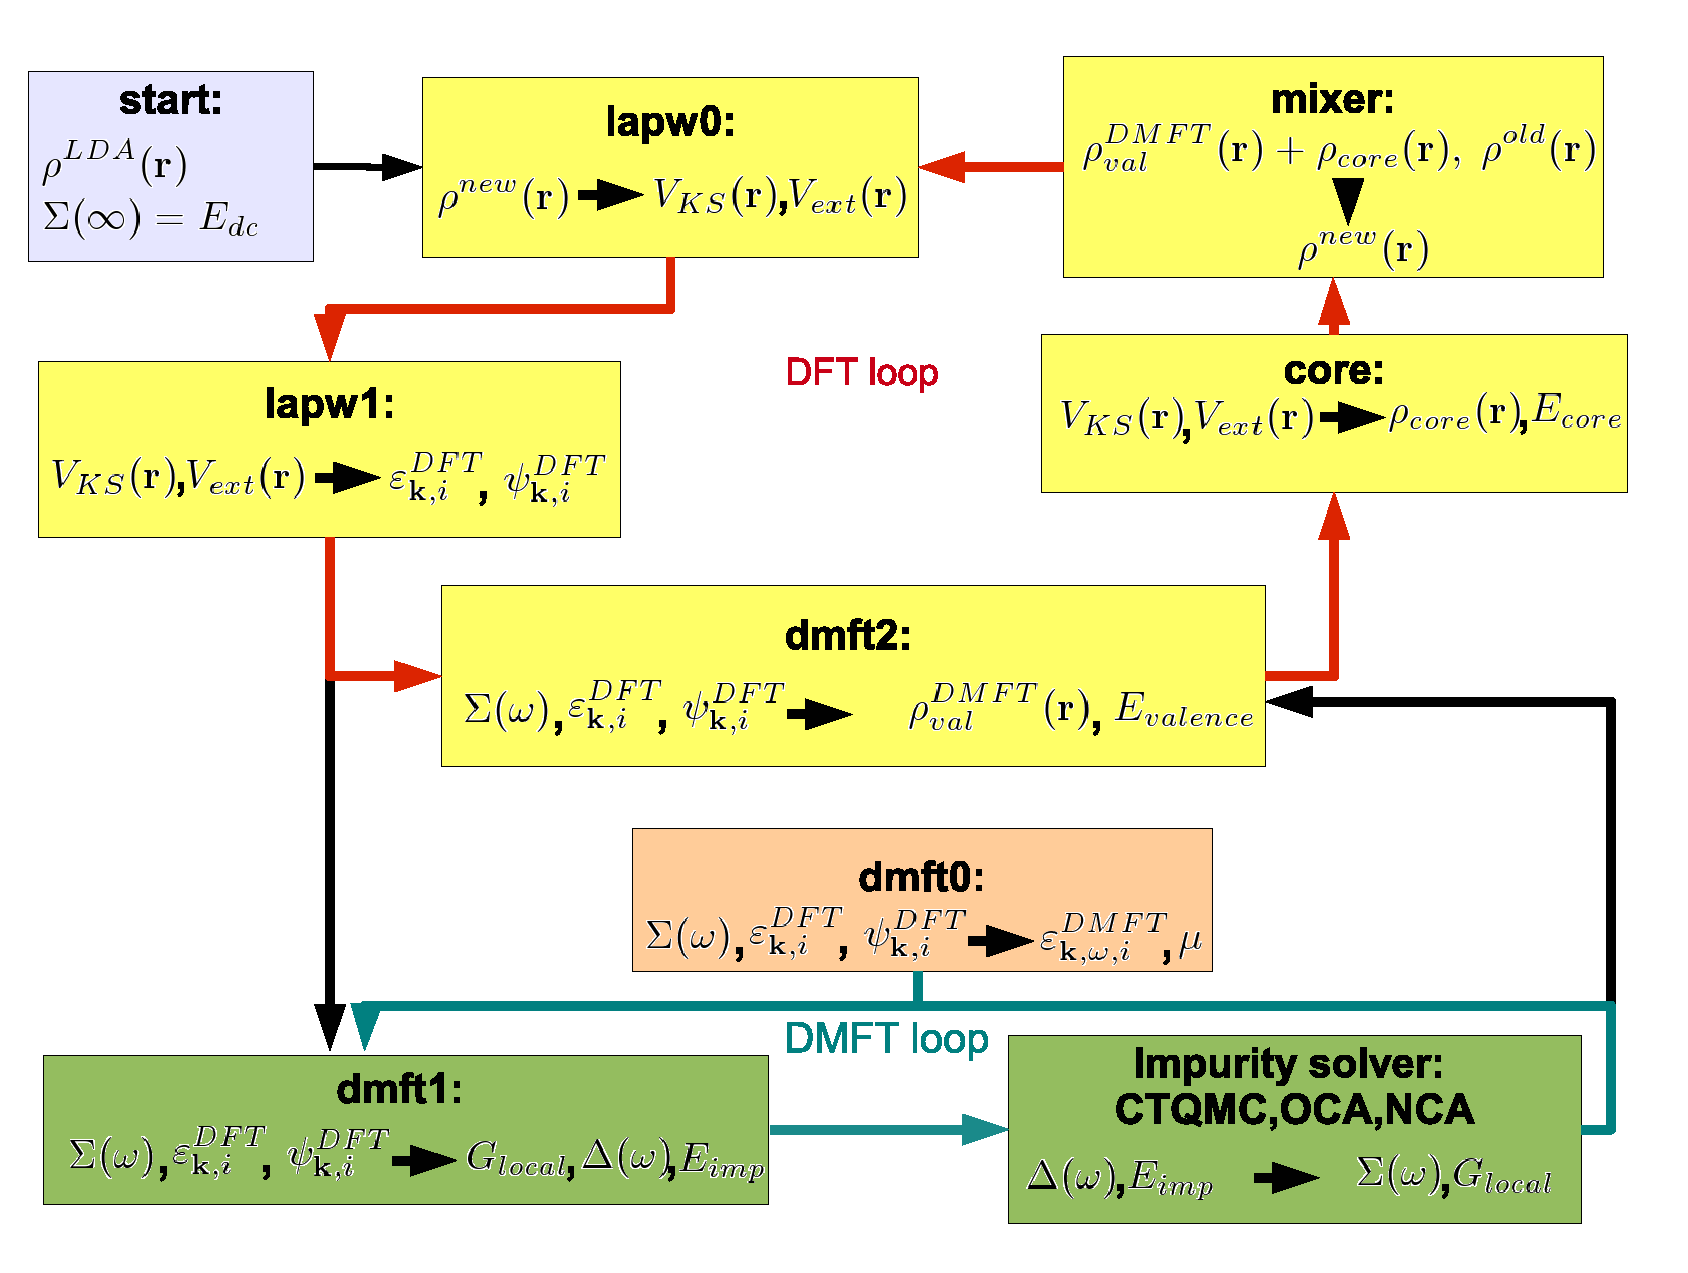
\includegraphics[width=1.0\linewidth]{lda+dmft-scheme1.eps}
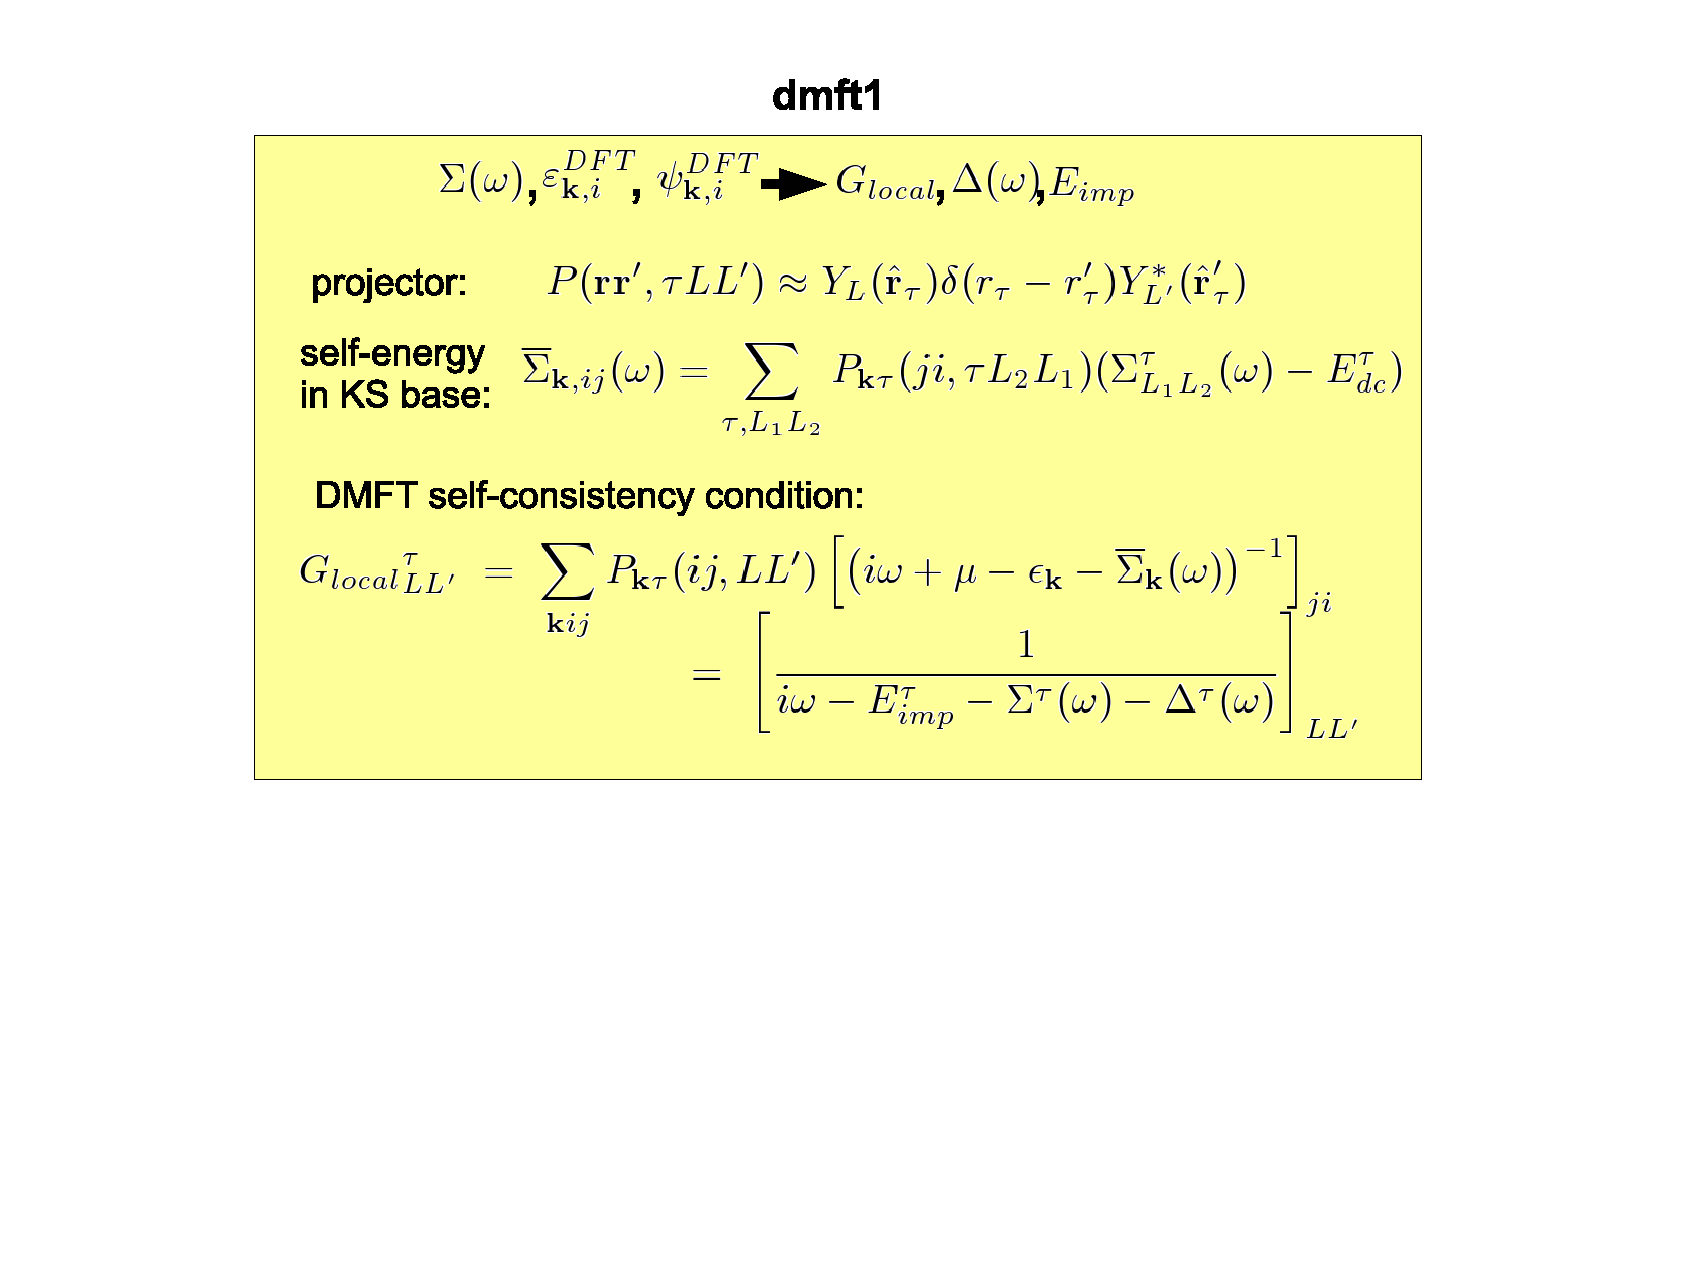
\includegraphics[width=1.0\linewidth]{lda+dmft-scheme2.eps}
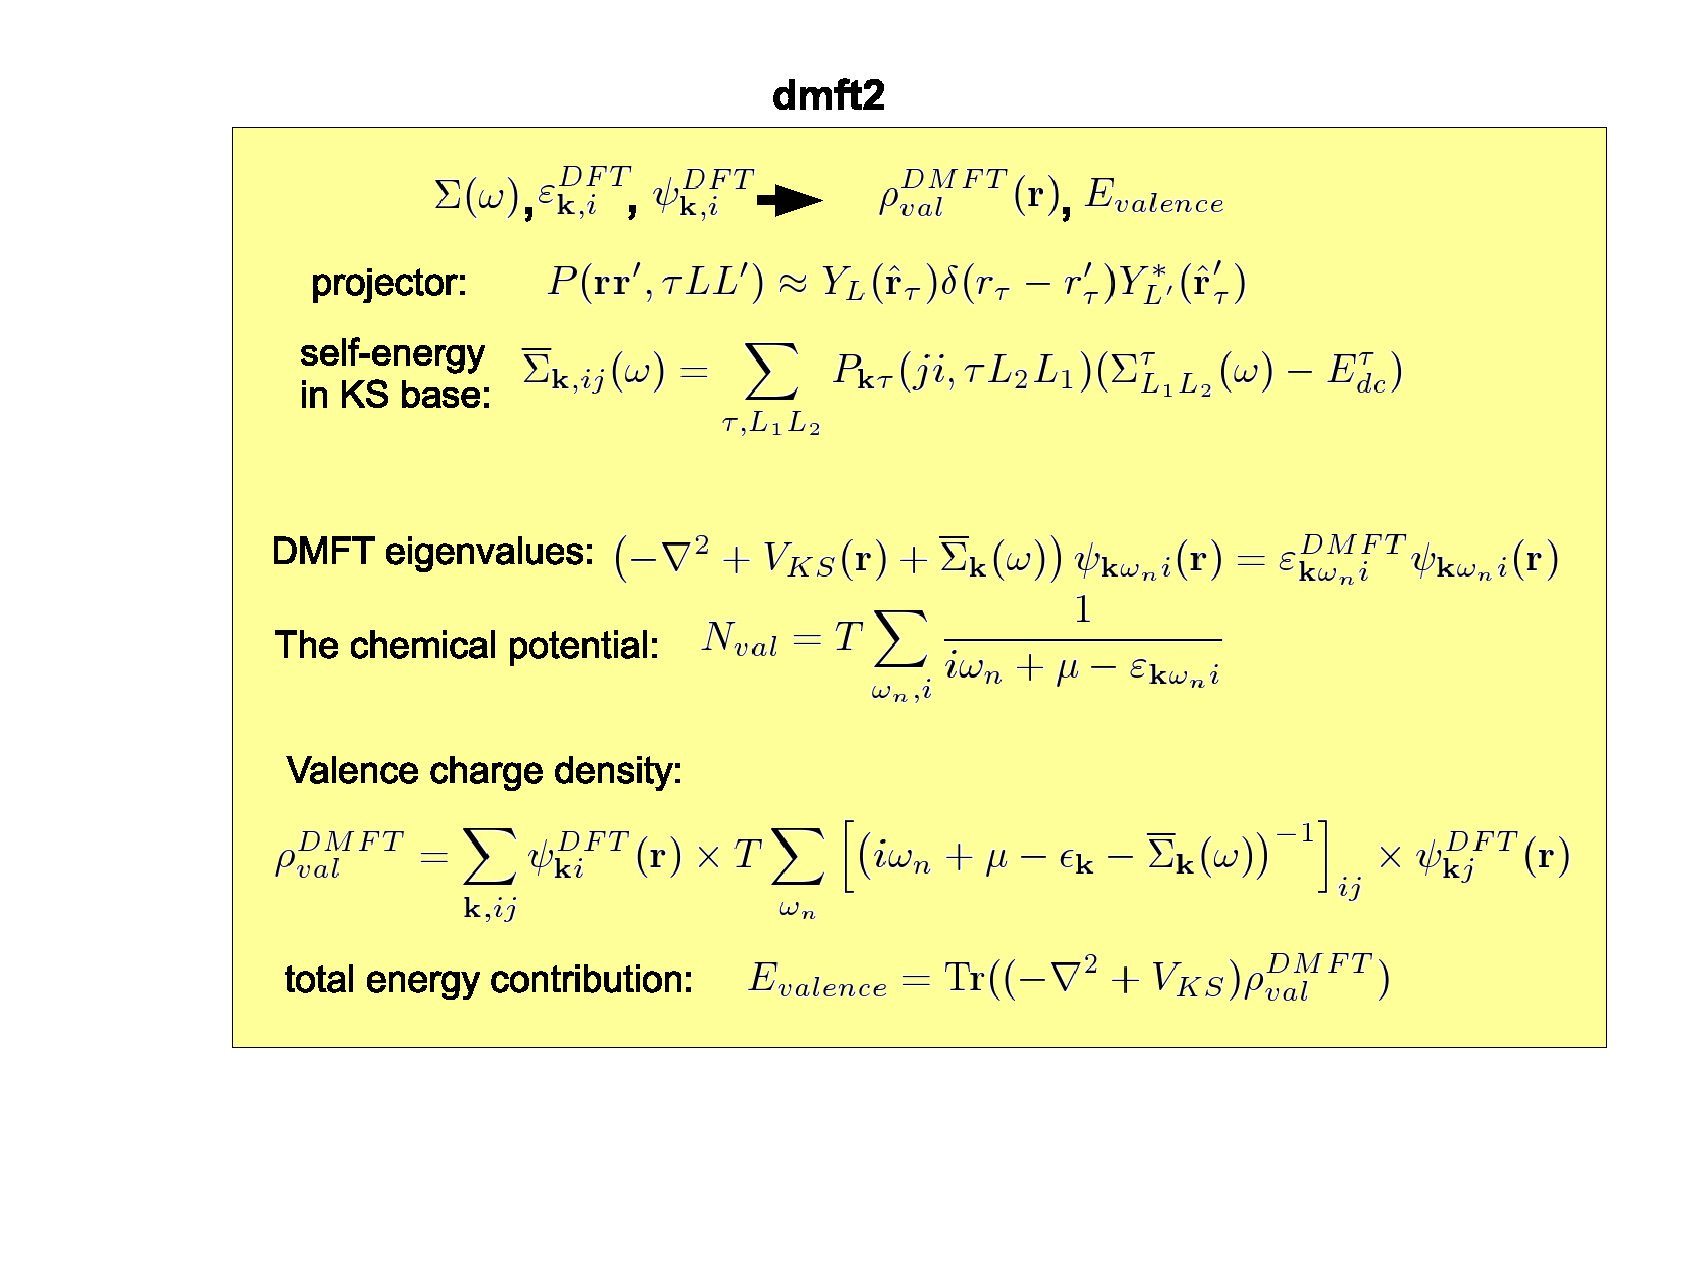
\includegraphics[width=1.0\linewidth]{lda+dmft-scheme3.eps}




\newslide

\begin{eqnarray}
G_{loc} &=& P_1 \left(\omega + \mu + \nabla^2 -V_{H}-\Sigma_{n-loc}^{GW}-E_1 \Sigma_{loc}\right)^{-1}\nonumber\\
W_{loc} &=& P_2 \left(V_C + \Pi_{n-loc}^{GW} + E_2 \Pi_{loc}\right)^{-1}\nonumber
\end{eqnarray}

\begin{eqnarray}
(\hat{P}_1\; O )(LL',\tau)\approx  \int d\vr d\vr' Y_L(\hat{\vr})\delta(r-r') Y_{L'}(\hat{\vr'})O(\vr,\vr')\nonumber\\
(\hat{E}_1\; O)(\vr\vr') \approx \sum_{L L'\tau} Y_L(\hat{\vr}_\tau )\delta(r_\tau
-r'_\tau) Y_{L'}(\hat{\vr}_\tau') O(LL',\tau)\nonumber
\end{eqnarray}

\begin{equation}
{\cal U}^{-1} = W_{loc}^{-1} + \Pi_{loc}\nonumber
\end{equation}

\begin{equation}
{\cal G}_0^{-1} = G_{loc}^{-1} + \Sigma_{loc}\nonumber
\end{equation}

\begin{eqnarray}
{\cal G}_0(\omega) \; {\cal U}(\omega)\\
G_{loc}(\omega),\; \Sigma_{loc}(\omega),\; W_{loc}(\omega),\; \Pi_{loc}(\omega)
\end{eqnarray}

\begin{eqnarray}
\Phi_{GW}(G,W)\\
\Phi_{DMFT}(G,W)
\end{eqnarray}

\begin{eqnarray}
G(\vr\vr')\\
W(\vr\vr')
\end{eqnarray}

\begin{eqnarray}
G_{loc}\\
W_{loc}\\
V_C\\
{\cal U}
\end{eqnarray}

\end{slide}
\end{document}
